% (c) Egor Osipov

\documentclass[a4paper,12pt]{article} % тип документа (report, book)
\usepackage[14pt]{extsizes}
\usepackage[left=2cm,right=2cm, top=2cm,bottom=2cm,bindingoffset=0cm]{geometry} % Настройки документа
\usepackage{pgfplots}
\usepackage{pgfplotstable}
\usepackage{tikz} 

%  Русский язык
\usepackage[T2A]{fontenc}			% кодировка
\usepackage[utf8]{inputenc}			% кодировка исходного текста
\usepackage[english,russian]{babel}	% локализация и переносы


% Математика
\usepackage{amsmath,amsfonts,amssymb,amsthm,mathtools} 

% Просто смайлики
\usepackage{wasysym}

%Вставка картинок
\usepackage{graphicx}
\graphicspath{./}
\DeclareGraphicsExtensions{.pdf,.png,.jpg}
\usepackage{float}

% Настройка абзацев
\usepackage{indentfirst}
%\setlength{\parindent}{5ex}
%\setlength{\parskip}{1em}

\begin{document} % начало документа

%Заговолок
\begin{titlepage}
\begin{center}
	\large{Московский физико-технический институт}\\
	\vspace{100px}
	\LARGE{Лабораторная работа № 3.3.4.}\\
	\LARGE{Эффект Холла в полупроводниках.}\\
	\vspace{30px}
	
\includegraphics[scale = 0.3]{fakt_logo.png}\\
\end{center}

\vfill
\begin{flushright}
	\text{Осипов Егор. Б03-005}\\
	\text{16.11.2021}\\
	\text{г. Долгопрудный}
\end{flushright}
\end{titlepage}

\newpage

\tableofcontents

\newpage

\section{Теория и вводные}

\subsection{Цель работы и используемые приборы.}

\textbf{Цель работы:} измерение подвижности и концентрации носителей заряда в полупроводниках.

\textbf{В работе испольщуются:} электромагнит с источником питания, амперметр, милиамперметр, милливеберметр, реостат, цифровой вольтметр, источник питания (1.5В), образцы легированного германия.

\subsection{Экспериментальная установка.}

\begin{figure}[H]\label{pic1}
	\center{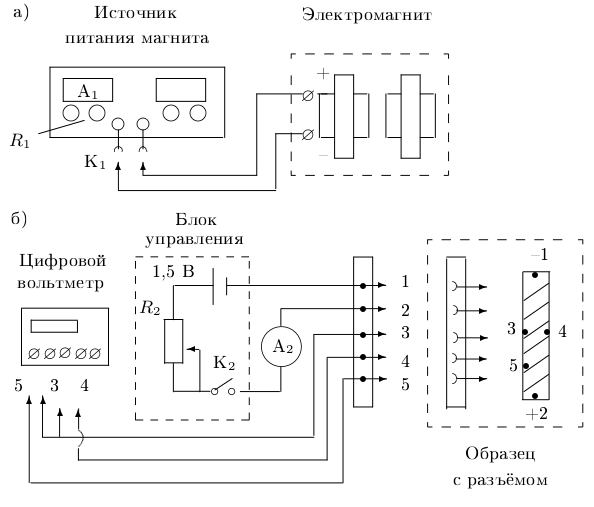
\includegraphics[scale=0.8]{pic1}}
 	\caption{Схема установки для исследования эффекта Холла в полупроводниках.}
\end{figure}

Схема установки для измерения ЭДС Холла представлена на рисунке \eqref{pic1}.

В зазоре электромагнита создаётся постоянное магнитное поле, величину которого можно менять с помощью регулятора $R_1$ источника питания электромагнита. Ток питания электромагнита измеряется амперметром $A_1$. Разьём $K_1$ позволяет менять направление тока в обмолках электромагнита.

Градуировка магнита проводится при помощи милливебермелра.

Образец из легированного германия, смонтированный в специальном держателе, подключается к источнику питания ($\simeq$ 1,5 В). При замыкании ключа $K_2$ вдоль длинной стороны образца течёт ток, величина которого регулируется реостатом $R_2$ и измеряется миллиамперметром $A_2$.

В образце с током, помещённом в зазор электромагнита, между контаклами 3 и 4 возникает разность потенциалов ($U_{34}$, которая измеряется с помощью цифрового вольтметра.

Иногда контакты 3 и 4 вследствие неточности поднайки не лежат на одной эквипотенциали, и тогда напряжение между ними связано не только с эффектом Холла, но и с омическим падением напряжения, вызванным протеканием основного тока через образец. Измеряемая разность потенциалов при одном направлении магнитного поля равна сумме ЭДС Холла и омического падения напряжения, а при друтом — их разности. В этом случае ЭДО Холла $\varepsilon_x$ может быть определена как половина алгебраической разности показаний вольтметра, полученных для двух противоположных направлений магнитного поля в зазоре. Знак измеряемого напряжения высвечивается на цифровом табло вольтметра.

Можно исключить влияние омического падения напряжения иначе, если при каждом токе через образец измерять напряжение между точками З и 4 в отсутствие магнитного поля. При фиксированном токе через образец это дополнительное к ЭДС Холла напряжение $U_0$ остаётся неизменным. От него следует (с учётом знака) отсчитывать величину ЭДС Холла:

\begin{equation}\label{eq1}
\varepsilon_x = U_{34} \pm U_0
\end{equation}

При таком способе измерения нет необходимости проводить повторные измерения с противоположным направлением магнитного поля.

По знаку $\varepsilon_x$ можно определить характер проводимости — электронный или дырочный. Для этого необходимо зналь направление тока в образце и направление магнитного поля.

Измерив ток I в образце и напряжение $U_{35}$ между контактами 3 и 5 в отсутствие магнитного поля, можно, зная параметры образца, рассчитать проводимость материала образца по формуле

\begin{equation}\label{eq2}
\sigma = \frac{I L_{35}}{U_{35} \textit{a l}}
\end{equation}

Где $L_{35}$ -- расстояние между контактами 3 и 5, \textit{a} -- толщина образца, \textit{l} -- его ширина.

\section{Ход работы.}

В работе предлагается исследовать зависимость ЭДС Холла от величины магнитного поля при различных токах через образец для определения константы Холла; определиль знак носителей заряда и проводимость материала образца.

1. Подготовим приборы к работе.

2. Проверим работу цепи питания образца. Ток через образец не должен
превышать 1 мА.

3. Проверим раболу цепи магнита. Определите диапазон изменения тока через магнит.

4. Прокалибруем электромагнит -- определите связь между индукцией В магнитного поля в зазоре электромагнита и током $I_m$ через обмотки магнита. Для этого с помощью милливеберметра снимем зависимость магнитного потока, $\Phi$ пронизывающего пробную катушку, находящуюся в зазоре, от тока $I_m$ ($\Phi = \text{BSN}$). Значение SN (произведение площади сечения контура катушки на число токов в ней) указано на держателе катушки.

5. Продевед измерение ЭДС Холла. Для этого втавим образец в зазор выключенного электромагнита и определим напряжение $U_0$ между холловскими контактами 3 и 4при минимальном токе через образец ($\simeq 0.2 \text{мА}$). Это напряжение $U_0$ вызвано несовершенством контактов 3, 4 и при фиксированном токе через образец остается неизменным. Значение $U_0$ с учетом значка следует принять за нулевое.

Включим электромагнит и снимем зависимость напряжения $U_{34}$ от тока $I_m$ через обмотки магнита при фиксированном токе через образец.

Проведем измерения $U_{34} = \textit{f }(I_m)$ при постоянном токе через образец для 6-8 его значений в интервале 0.2-1 мА. При каждом новом значении тока через образец величина $U_0$ будет иметь свое значение.

При максимальном токе через образец ($\simeq 1$ мА) $U = \textit{f }(I_m)$ при другом направлении магнитного поля.

6. Определим знак носителей в образце. Для этого необходимо знать направление тока через образец, направление магнитного поля и знак ЭДС Холла.

Направление тока в образце показано знаками «+» и «-» на рисунке \eqref{pic1}. Направление тока в обмотках электромагнита при установке разъёма $K_1$ в положение I показано стрелкой на торце магнита.

Сфотографируем образец. Укажем на рисунке направления тока, магнитного поля и отклонение носителей. По знаку ($\pm$) на клеммах цифрового вольтметра определите характер проводимости.

7. Для определение удельной проводимости удалим держатель с образцом из зазора. Подлкючим к клеммам «$H_x$» и «$L_x$» вольтметра поленциальные концы 3 и 5. Измерим падение напряжения между ними при токе через образец 1 мА.

8. Запишем характеристики приборов и параметры образца $L_{35}$, \textit{a, l}, указанные на держателе.

\section{Обработка результатов.}

\subsection{Градуировка электромагнита.}

\begin{table}[H]
\caption{\label{tab:canonsummary} Зависимость индукции магнитного поля в зазоре электромагнита B от силы тока $I_m$.}
\begin{center}
\begin{tabular}{|c|c|c|c|c|c|c|c|}
\hline
$\phi$, мВб & 6.5 & 6.3 & 5.8 & 4.8 & 3.7 & 1.9\\
\hline
$I_m$, А & 1.58 & 1.41 & 1.15 & 0.88 & 0.66 & 0.32\\
\hline
B, мТл & 866.67 & 840.00 & 773.33 & 640.00 & 493.33 & 253.33\\
\hline
\end{tabular}
\end{center}
\label{table1:ref}
\end{table}

\begin{figure}[H]\label{gr1}
	\center{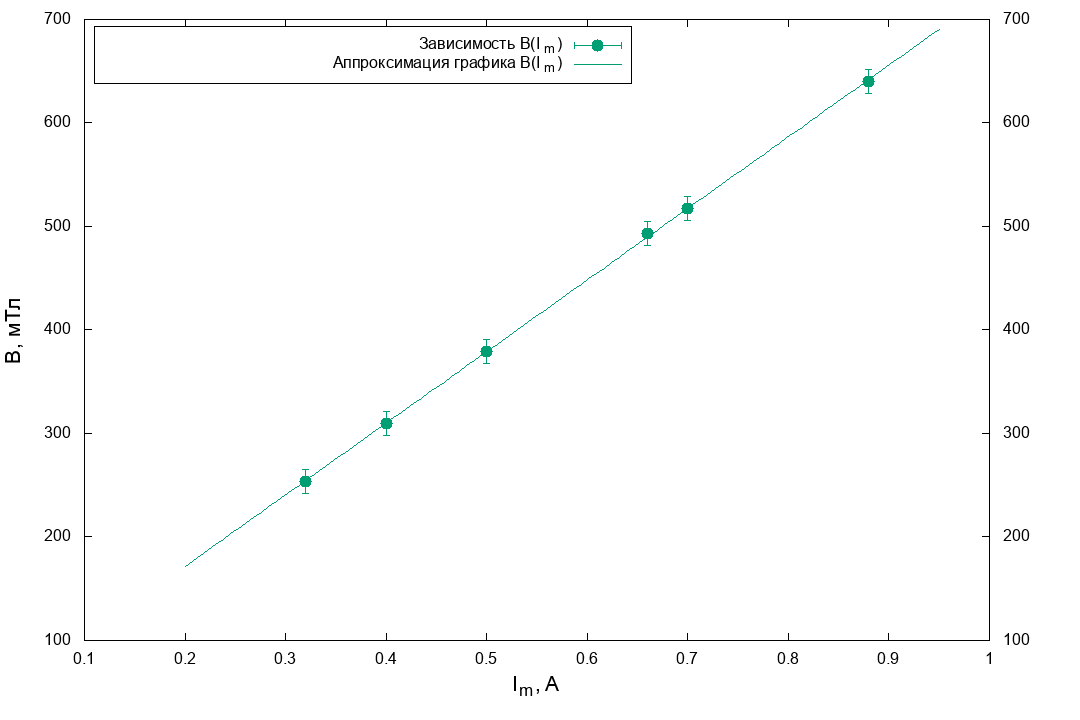
\includegraphics[scale=0.6]{gr1}}
 	\caption{Зависимость индукции магнитного поля в зазоре эектромагнита B от силы тока $I_m$}
\end{figure}

\subsection{Измерение ЭДС Холла.}

\begin{table}[H]
\caption{\label{tab:canonsummary} Рассчет величины ЭДС Холла.}
\begin{center}
\begin{tabular}{|c|c|c|c|c|c|c|c|}
\hline
I = 0.3 мА&&&&&&\\
\hline
$I_m$, А & 0.31 & 0.60 & 0.88 & 1.03 & 1.22 & 1.57 \\
\hline
B, мТл & 247.77 & 448.39 & 642.09 & 745.86 & 877.30 & 1119.42 \\ 
\hline
$\varepsilon_x$, мВ & -0.04 & -0.07 & -0.10 & -0.12 & -0.13 & -0.14 \\ 
\hline
I = 0.4 мА&&&&&&\\
\hline
$I_m$, А & 0.30 & 0.60 & 0.81 & 1.06 & 1.27 & 1.57 \\
\hline
B, мТл & 240.85 & 448.39 & 593.66 & 766.61 & 911.89 & 1119.42 \\
\hline
$\varepsilon_x$, мВ & -0.05 & -0.09 & -0.12 & -0.15 & -0.17 & -0.18 \\ 
\hline
I = 0.5 мА&&&&&&\\
\hline
$I_m$, А & 0.33 & 0.60 & 0.74 & 0.93 & 1.31 & 1.57 \\ 
\hline
B, мТл & 261.60 & 448.39 & 545.24 & 676.68 & 939.56 & 1119.42\\ 
\hline
$\varepsilon_x$, мВ & -0.06 & -0.12 & -0.14 & -0.17 & -0.21 & -0.23 \\
\hline
I = 0.6 мА&&&&&&\\
\hline
$I_m$, А & 0.22 & 0.40 & 0.61 & 0.95 & 1.36 & 1.56 \\ 
\hline
B, мТл & 185.51 & 310.03 & 455.30 & 690.51 & 974.15 & 1112.51 \\ 
\hline
$\varepsilon_x$, мВ & -0.05 & -0.09 & -0.14 & -0.21 & -0.26 & -0.28 \\ 
\hline
I = 0.7 мА&&&&&&\\
\hline
$I_m$, А & 0.27 & 0.61 & 0.90 & 1.20 & 1.37 & 1.57 \\
\hline
B, мТл & 220.09 & 455.30 & 655.92 & 863.46 & 981.07 & 1119.42 \\ 
\hline
$\varepsilon_x$, мВ & -0.07 & -0.16 & -0.23 & -0.28 & -0.30 & -0.32 \\
\hline
I = 0.8 мА&&&&&&\\
\hline
$I_m$, А & 0.30 & 0.60 & 0.72 & 1.05 & 1.25 & 1.57 \\
\hline
B, мТл & 240.85 & 448.39 & 531.40 & 759.69 & 898.05 & 1119.42 \\ 
\hline
$\varepsilon_x$, мВ & -0.09 & -0.19 & -0.22 & -0.30 & -0.33 & -0.37 \\
\hline
I = 0.9 мА&&&&&&\\
\hline
$I_m$, А & 0.33 & 0.60 & 0.81 & 1.07 & 1.37 & 1.56\\
\hline
B, мТл & 261.60 & 448.39 & 593.66 & 773.53 & 981.07 & 1112.51 \\ 
\hline
$\varepsilon_x$, мВ & -0.18 & -0.27 & -0.34 & -0.41 & -0.46 & -0.48 \\ 
\hline
I = 1 мА&&&&&&\\
\hline
$I_m$, А & 0.33 & 0.60 & 0.76 & 1.06 & 1.32 & 1.57 \\ 
\hline
B, мТл & 261.60 & 448.39 & 559.07 & 766.61 & 946.48 & 1119.42\\ 
\hline
$\varepsilon_x$, мВ & -0.19 & -0.30 & -0.36 & -0.45 & -0.50 & -0.53 \\ 
\hline
\end{tabular}
\end{center}
\label{table1:ref}
\end{table}

%\begin{table}[H]
%\caption{\label{tab:canonsummary} Расчет величины ЭДС Холла}
%\begin{center}
%\begin{tabular}{|c|c|c|c|c|c|c|c|}
%\hline
%I = 0.2 мА & \\
%\hline
%0.15 & -0.023 \\ \hline
%0.25 & -0.016 \\ \hline
%0.35 & -0.009 \\ \hline
%0.45 & -0.002 \\ \hline
%0.55 & 0.003 \\ \hline
%0.6 & 0.007 \\ \hline
%0.65 & 0.01 \\ \hline
%0.75 & 0.015 \\ \hline
%0.85 & 0.022 \\ \hline
%0.95 & 0.025 \\ \hline
%1.05 & 0.031 \\ \hline
%1.15 & 0.034 \\  \hline
%1.25 & 0.039 \\ \hline
%1.35 & 0.042 \\  \hline
%1.45 & 0.045 \\ \hline
%1.55 & 0.047 \\ \hline
%1.65 & 0.049 \\ \hline
%1.75 & 0.051 \\ \hline
%1.85 & 0.053 \\ \hline
%1.95 & 0.054 \\ \hline
%2.05 & 0.055 \\ \hline
%2.09 & 0.056 \\ \hline
%\hline
%\end{tabular}
%\end{center}
%\label{table1:ref}
%\end{table}
%
%\begin{table}[H]
%\begin{center}
%\begin{tabular}{|c|c|c|c|c|c|c|c|}
%\hline
%I = 0.4 мА & \\
%\hline
%0.15 & -0.046\\ \hline 
%0.25 & -0.033\\ \hline 
%0.35 & -0.021\\ \hline 
%0.45 & -0.007\\ \hline 
%0.55 & 0.004\\ \hline 
%0.65 & 0.017\\ \hline 
%0.75 & 0.028\\ \hline 
%0.85 & 0.038\\ \hline 
%0.95 & 0.048\\ \hline 
%1.05 & 0.057\\ \hline 
%1.15 & 0.065\\ \hline 
%1.25 & 0.073\\ \hline 
%1.35 & 0.078\\ \hline 
%1.45 & 0.084\\ \hline 
%1.55 & 0.088\\ \hline 
%1.65 & 0.092\\ \hline 
%1.75 & 0.095\\ \hline 
%1.85 & 0.098\\ \hline 
%1.95 & 0.101\\ \hline 
%2.05 & 0.104\\ \hline 
%\hline
%\end{tabular}
%\end{center}
%\label{table1:ref}
%\end{table}
%
%\begin{table}[H]
%\begin{center}
%\begin{tabular}{|c|c|c|c|c|c|c|c|}
%\hline
%I = 0.6 мА & \\
%\hline
%0.15 & -0.046\\ \hline 
%0.25 & -0.033\\ \hline 
%0.35 & -0.021\\ \hline 
%0.45 & -0.007\\ \hline 
%0.55 & 0.004\\ \hline 
%0.65 & 0.017\\ \hline 
%0.75 & 0.028\\ \hline 
%0.85 & 0.038\\ \hline 
%0.95 & 0.048\\ \hline 
%1.05 & 0.057\\ \hline 
%1.15 & 0.065\\ \hline 
%1.25 & 0.073\\ \hline 
%1.35 & 0.078\\ \hline 
%1.45 & 0.084\\ \hline 
%1.55 & 0.088\\ \hline 
%1.65 & 0.092\\ \hline 
%1.75 & 0.095\\ \hline 
%1.85 & 0.098\\ \hline 
%1.95 & 0.101\\ \hline 
%2.05 & 0.104\\ \hline 	
%\hline
%\end{tabular}
%\end{center}
%\label{table1:ref}
%\end{table}

\newpage

\begin{figure}[H]\label{gr2}
	\center{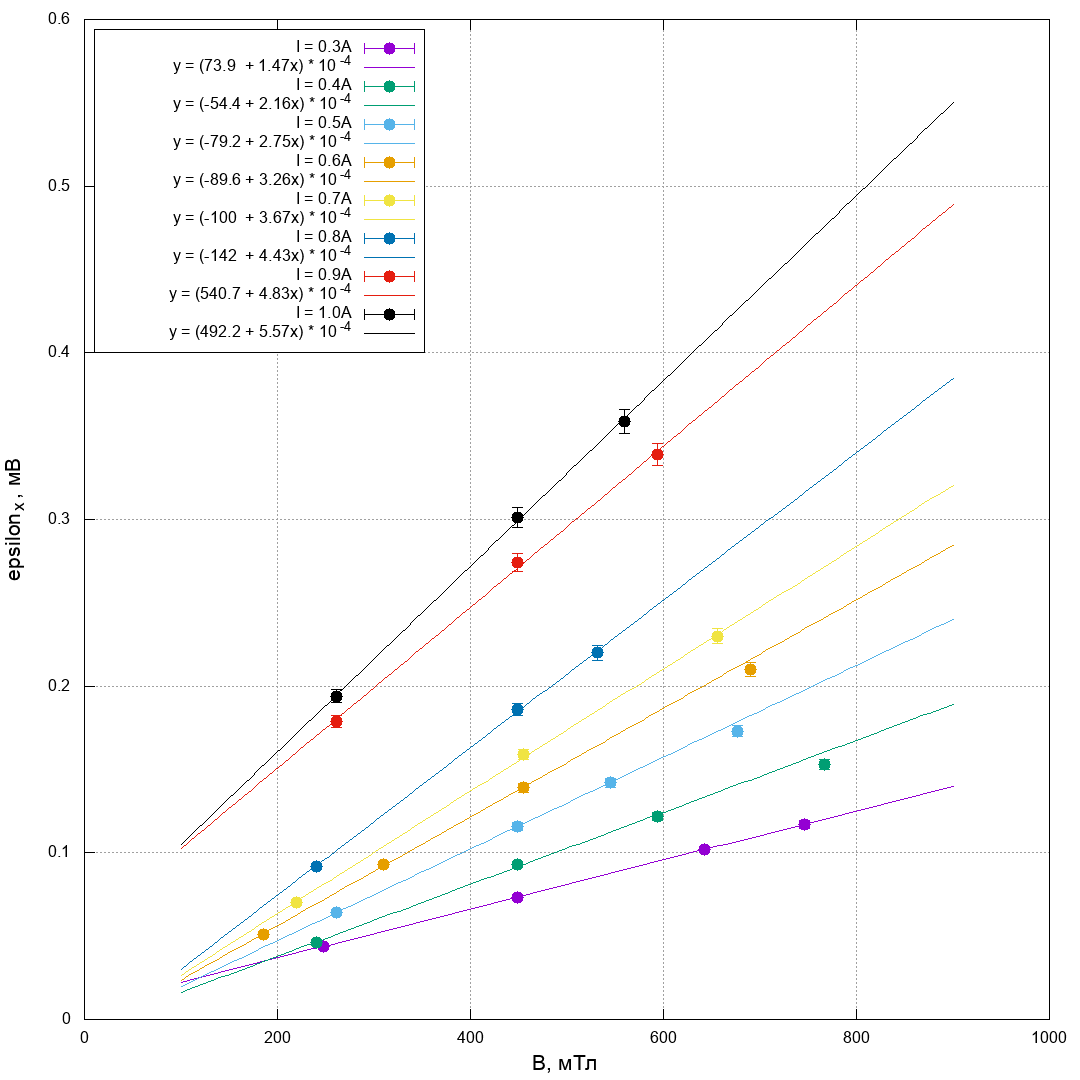
\includegraphics[scale=0.6]{gr2}}
 	\caption{Зависимость величины ЭДС Холла $\varepsilon_x$ от индукции поля в зазоре электромагнита.}
\end{figure}

\begin{figure}[H]\label{gr3}
	\center{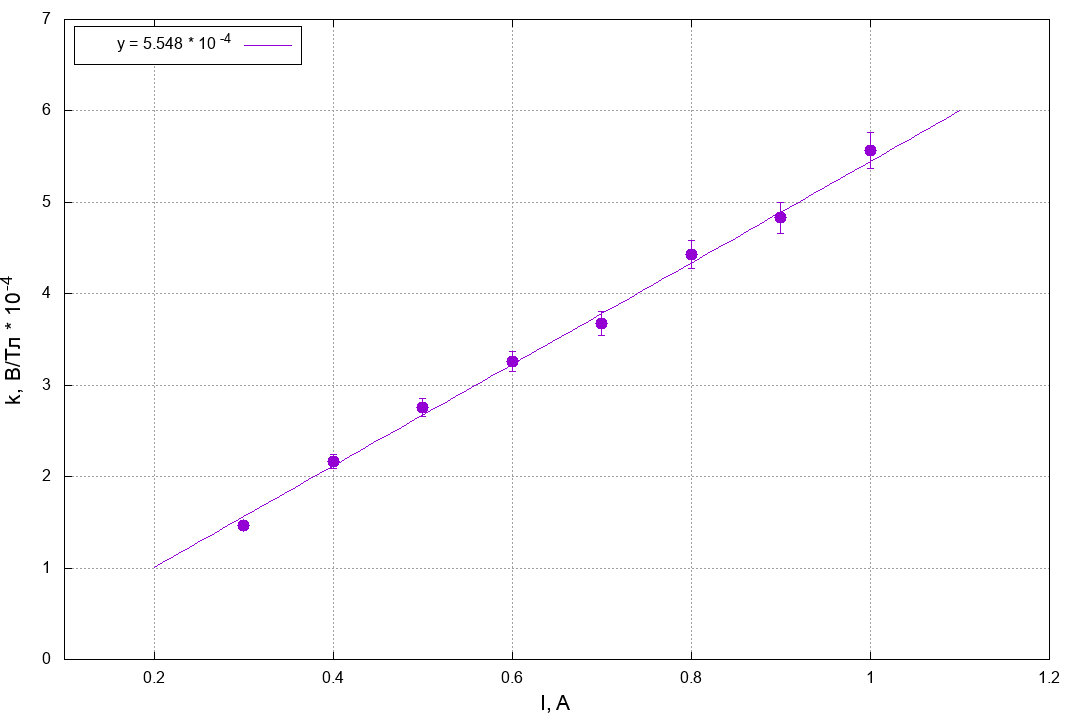
\includegraphics[scale=0.6]{gr3}}
 	\caption{Зависимость коэффициента $k = \vartriangle \varepsilon_x / \vartriangle B$ от силы тока I.}
\end{figure}

\begin{equation*}
\varepsilon_x = -R_x \frac{I B}{a} \Rightarrow k = -R_x \frac{I}{a} \Rightarrow R_x = - a\frac{k}{I}
\end{equation*}

Отсюда очевидно, что $R_x = 0.83 \text{см}^3/\text{Кл}$.

\begin{equation*}
\sigma = \frac{I L_{35}}{U_{35} a l}
\end{equation*}

И в конечном итоге $\sigma = 701.11 \text{Ом/м}$

\section{Вывод.}

В результате эксперимента мы измерили постоянную Холла, которая оказалась $R_x = 0.83 \text{см}^3/\text{Кл}$, из которой мы получили удельную проводимость легированного германия: $\sigma = 701.11 \text{Ом/м}$

\end{document} % конец документа